% author: Tomas Trnka
% mail: tomas@trnkatomas.eu
% date: 2013-07-04

\documentclass[a4paper,10pt]{article}
%\usepackage[czech]{babel}
%\usepackage[T1]{fontenc}
\usepackage[hmargin=2.2cm,vmargin=2.2cm]{geometry}
\usepackage[utf8x]{inputenc}
\usepackage{fancyhdr}
\usepackage{fancyvrb}
\usepackage{amsmath, amsthm, amssymb}
\usepackage{float}
\usepackage{enumerate}
\usepackage{tikz}
\usepackage{hyperref}
\pagestyle{fancy}
\headheight 15pt
\lhead{Crpyto, Fall 2014}
\rhead{Tomas Trnka}
\newcommand{\set}[1]{\ensuremath{\left\lbrace #1 \right\rbrace}}
\newcommand{\role}[1]{\ensuremath{\left\langle #1 \right\rangle}}
\newcommand{\cara}{\begin{center}\rule{140mm}{.2mm}\end{center}}
\newcommand{\mI}{\ensuremath{^\mathcal{I}}}
\newcommand{\Tbox}[1]{\ensuremath{\mathcal{T}}-Box#1}
\newcommand{\Abox}[1]{\ensuremath{\mathcal{A}}-Box#1}
\newcommand{\mC}[1]{\ensuremath{\mathcal{#1}}}
\newcommand{\Tc}{\ensuremath{\mathcal{T}_c}}
\newcommand{\qb}[1]{\ensuremath{\vert{#1}\rangle}}
\begin{document}
\section*{Hash functions and MACs}
\begin{enumerate}
\item authentication - one of the most important applications is the internet comunication when we would like to communicate fx. with the banks, the adversary can certainly change the message, intercept it and his goal is to persuade B that the message he is sending was sent by A.

\item where we can use the hash and MAC?
\begin{itemize}
\item[]\textbf{Adversary can only change the message}\\
a  typical  application  wouldbe a user that computes an authenticatorsfor the datam.  He storesmin some insecure location, but brings the authenticator with him insecure storage (say, on a chipcard).  Later, he wants to check that thedata  has not  been  changed.   Such  systems  can be  built  fromcrypto-graphic hash functions.
\item[]\textbf{Adversary can change both message and authenticator}\\
This will bethe case when a sender communicates with a receiver over an insecurechannel.  The are two subcases:Sender and receiver share a secret key:In this case, authentica-torsis computed from both datamand the secret keyk.m;sissent on the channel, andm0;s0is received.  Then the receiver can,using thesamekeyk, test ifm0;s0look OK. Of course, this shouldalways be the case ifm0;s0=m;s,and we hope that anyone whodoes not knowkcannot come up with a fake pairm0;s0that thereceiver would accept.  Such systems can be built usingMessageAuthentication Codes(MAC's) also calledKeyed Hash Functions.
\end{itemize}
\end{enumerate}
\subsection*{Hash functions}
\begin{itemize}
\item defined as generator $\mathcal{H} \text{ is } h: \{0,1\}^* \rightarrow \{0,1\}^k$, there is no key so we can assume that everyone (adversary included knows everything even about this function)
\item message digest,  fingerprint - one reason why we wanted limited length is that is much easier to store rather small amounts of data securely
\item possible attacks for the adversary would be to came up with \textit{second preimage} or the whole pair that creates a collision $h(m)=h(m')$.
\item 
\textbf{Definition 1} Consider the game where we run $\mathcal{H}$ on input k to get function h. We give h as input to adversary algorithm A, who outputs 2 strings m,m'. We say that A has success if $m \neq m'$ and $h(m) = h(m')$. We say that $\mathcal{H}$ is collision intractable, if any polynomial-time A has success with negligible probability (as a function of k).
\item 
\textbf{Theorem 1} If there exists a collision-intractable hash function generator $\mathcal{H}$ producing functions with finite input length $m > k$ and $t(k),\varepsilon(k)$ security, then there exists a collision-intractable generator $\mathcal{H}$ that produces functions taking arbitrary length inputs.\\
(This is basically Merkele-Damgaard theorem and it would be especially shameful to fail to explain it, moreover the proof is kind of understandable but takes a lot of time - ideal candidate to present!)
\item
\textbf{Theorem 2} Given function h, and assume that it is possible to sample input values to h causing the outputs to be uniformly random in ${0,1}^k$. Then a collision for h can be found with constant probability in time corresponding to $2^{\frac{k}{2}}$ evaluations of h. (Birthday paradox)
\item there may be some history and real world example, that in real world we normally don't have any sort of generator but simple functions h like MD5, SHA-1, SHA-3 even standardised by the NIST
\item Random oracle model - it would be great if we could consider hash function as a random oracle, because there would not be any other attack than brute force  -- unfortunately it is not the case, There might be special attacks against \textit{h}.
\end{itemize}

\subsection*{Message authentication codes -- MACs}
\begin{itemize}
\item A secret-key authentication system consists of three probabilistic algorithms \textit{(G,A,V)}. \textit{G} which outputs a key \textit{K}, usually it works by simply choosing K as a random bit string of a certain length. Algorithm \textit{A} gets input a message \textit{m} and the key \textit{K} and produces an authenticator value $s = A_K(m)$. Finally
algorithm \textit{V} gets as input an authenticator \textit{s}, a message \textit{m} and key \textit{K}, and
outputs $V_K(s,m)$ which is equal to accept or reject. It is required that we
always have $V_K(A_K(m),m) = accept$.
\end{itemize}
\subsubsection*{security of secret-key systems}

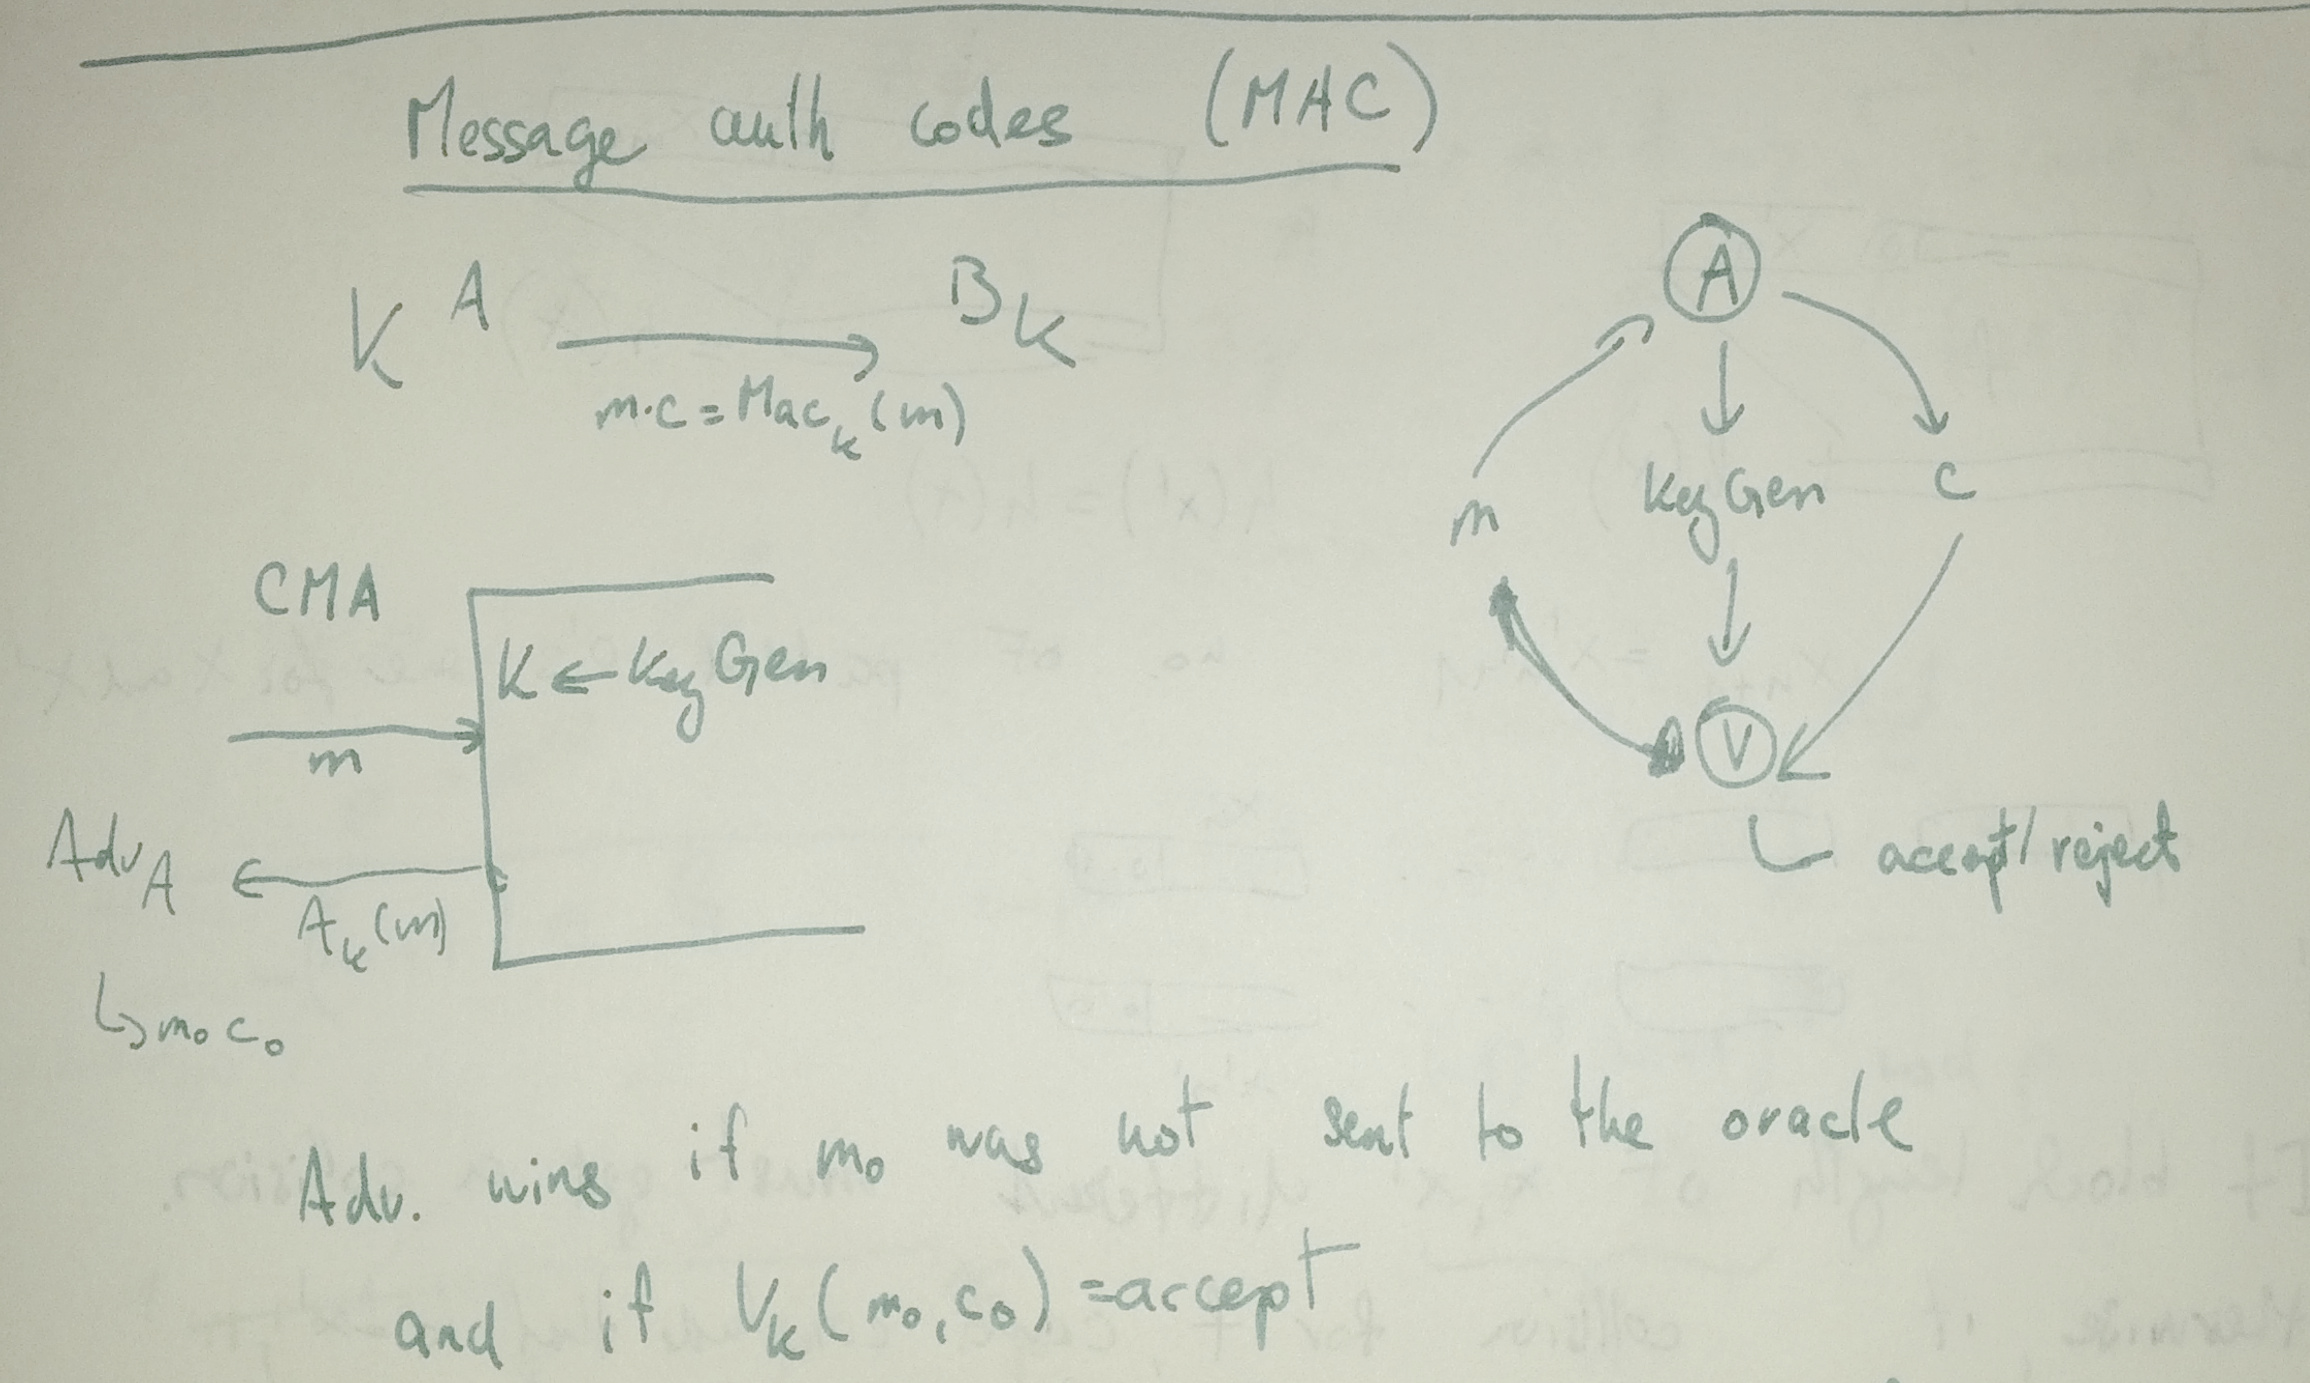
\includegraphics[width=\textwidth]{MAC.jpg}
\begin{itemize}
\item adversary can select as many m he would like to, the only condition is that at the end he has to produce the pair that will be validated
\item \textbf{Definition 2} (CMA Security of MACs) We say that a MAC sheme
is $(t,q,\varepsilon)$ CMA-secure if any adversary that runs in time at most \textit{t} and asks at most \textit{q} queries, wins the above game with probability at most $\varepsilon$.
\item \textbf{CBC-MAC}\\
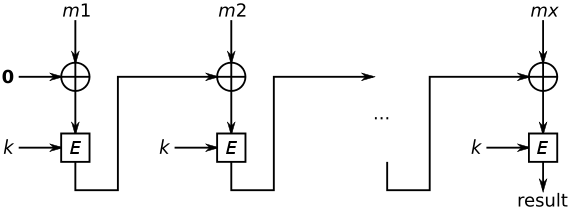
\includegraphics[width=0.9\textwidth]{CBC-MAC.png}
The CBC-MAC scheme follows from the CBC scheme for ciphers. There are some limitations for example the length of the input does not necessary have to be the multiple of the \textit{k} but we can use some padding scheme to solve it. To ensure ourselves we have to prepend the length of the message and then apply the whole procedure. If we append it, it won't work (example solverd in exercise 11).
We can also ensure the security by using normal CBC-MAC and then MAC the result under different key ECBC (CMAC).
\item \textbf{HMAC}\\
based on SHA-1: the key is a random 512-bit string K. The scheme uses two 512 bit constants ipad =3636...36, opad = 5C5C...5C, in HEX notation. Then we define
$$
HMAC_K(m) = SHA1( (K \oplus opad) || SHA1((K \oplus ipad)||m) )
$$



\end{itemize}



\end{document}